% presentation
\documentclass[compress]{beamer}

% handout
%\documentclass[handout]{beamer}

\mode<beamer>{
  \usetheme{Frankfurt}
  \mode<presentation>
}

\mode<handout>{
  \usepackage{pgfpages}
  \pgfpagesuselayout{2 on 1}[a4paper]
}
\usepackage{fancyvrb}
\usepackage{tikz}
\usetikzlibrary{mindmap,trees,3d,calc}


% other themes
%\usepackage{beamerthemeWarsaw}
%\usepackage{beamerthemeBoadilla}
%\usepackage[compress]{beamerthemeSingapore}


% layout settings
\setbeamertemplate{blocks}[rounded][shadow=false]
\setbeamertemplate{navigation symbols}{}
\setbeamersize{text margin left = 4mm}
\setbeamersize{text margin right = 4mm}
\setbeamercovered{transparent}

% other packages
%\usetheme[Boadilla]{}
\usepackage{calc}
\usepackage[ruled]{algorithm2e}
\usepackage{stmaryrd}
%

%\usepackage{tabularx,booktabs}
\usepackage{booktabs}
%\useinnertheme{rounded}
\usecolortheme{dolphin}
\usecolortheme{rose}
%\setbeamercolor{title}{fg=black,bg=white!80!black}
\setbeamercolor{title}{fg=black,bg=white!80!blue}
\usefonttheme[onlysmall]{structurebold}


\newcommand{\crystal}[5]{%
  \draw[->, >=latex, #5] (#1) --+ (#2);%
  \draw[->, >=latex, #5] (#1) --+ (#3);%
  \draw[->, >=latex, #5] (#1) --+ (#4);%
}

\newcommand{\fillcrystal}[5]{%
  \filldraw[fill=red!25,draw=red!35,opacity=0.5]
%  (0,0) + (1,0) -- (0,0) --++ (0,1) --+ (1,0);
  (#1) +(#2) -- (#1) --++ (#3) -- +(#2) ;%
  \filldraw[fill=red!45,draw=red!35,opacity=0.5]
  (#1) +(#3) -- (#1) --++ (#4) -- +(#3) ;%
  \filldraw[fill=red!65,draw=red!35,opacity=0.5]
  (#1) +(#4) -- (#1) --++ (#2) -- +(#4) ;%
  \draw[->, >=latex, #5] (#1) --+ (#2);%
  \draw[->, >=latex, #5] (#1) --+ (#3);%
  \draw[->, >=latex, #5] (#1) --+ (#4);%
}

\newcommand{\filldirection}[5]{%
  \filldraw[fill=red!25,draw=red!35,opacity=0.5]
%  (0,0) + (1,0) -- (0,0) --++ (0,1) --+ (1,0);
  (#1) +(#2) -- (#1) --++ (#3) -- +(#2) ;%
  \filldraw[fill=red!45,draw=red!35,opacity=0.5]
  (#1) +(#3) -- (#1) --++ (#4) -- +(#3) ;%
  \filldraw[fill=red!65,draw=red!35,opacity=0.5]
  (#1) +(#4) -- (#1) --++ (#2) -- +(#4) ;%
  \draw[->, >=latex, #5] (#1) --+ (#2);%
  \draw[->, >=latex, #5] (#1) --+ (#3);%
  \draw[->, >=latex,color=red, very thick] (#1) --+ (#4);%
}



\usepackage{colortbl}

\usepackage{listings}


\definecolor{lightgray}{gray}{0.9}
\definecolor{lightergray}{gray}{0.92}
\definecolor{mygreen}{rgb}{0.1,0.9,0.3}
\definecolor{commentgreen}{rgb}{0.3,1,0.5}

\definecolor{lightgray}{gray}{0.9} \lstset{backgroundcolor=\color{lightgray}}
\lstdefinelanguage{rock}{morekeywords=
{mean,std,hist,save,load,rotate,min,max,get,tensor,loadTensor,
scale,union,delete,degree,kernel,gethw,getparameter,bandwidth,
symmetry,Miller,Miller2quat,uniformODF,unimodalODF,fibreODF,xvector,yvector,zvector,
loadPoleFigure,PoleFigure,plot,plotpdf,plotipdf,calcODF,calcKernel,calcTensor,calcMDF,calcMisorientation,
vector3d,cross,norm, dot,sum,savefigure,plotDiff,calcerror,
quaternion,idquaternion,dist,Laue,length,angle,add,subGrid,refine,GridLength,getResolution,getRho,
polar,S2Grid,santafee,mix2,modalorientation,fourier,textureindex,entropy,volume,
surface, fibrevolume,uiimport,scatter,cif2symmetry,remove_outlier,
simulatePoleFigure,SimulateEBSD,grainfun,hold,getFundamentalRegion,symvec,
FourierODF,find_outlier,bar,copyproperty,plotspatial,hasholes,principalcomponents,
hullprincipalcomponents,loadEBSD,calcGrains,plotboundaries,plotodf,plotspatial,area,
aspectratio,grain,grainfun,grainsize,get,plotgrains,plotellipse,plotsubfractions,plotboundary,
hasholes,hassubfraction,hullarea,hullcentroid,hullperimeter,centroid,borderlength,
deltaarea,equivalentperimeter,perimeter,joincount,link,misorientation,neighbours,
paris,shapefactor,toebsd,rotation,axis,Euler,symmetrise,orientation,eq,inverse,BinghamODF,set,
project2FundamentalRegion,annotate,plotAngleDistribution,volumeCompressibility,
YoungsModulus, shearModulus, linearCompressibility, ChristoffelTensor,
velocity,
PoissonRatio,plotx2north,plotx2east,setpref,import,loadOrientation,loadVector3d,brassOrientation,double,EinsteinSum,directionalMagnitude,inv},
sensitive=false, morestring=[b][\emph]', moredelim=[is][\alert]{/+}{+/},
morecomment=[s][\emph]{<options}{>}, morecomment=[l]{\%},
commentstyle=\color{darkgray}\itshape }

\lstset{language=rock}
\lstset{emph={symmetries,concentration},emphstyle={\bf \color{white!25!black}}}


% \definecolor{mydarkgray}{rgb}{0.25,0.3,0.25}
% \lstset{
%   language=Matlab,
%   escapeinside="",
%   keywordstyle=\color{black},
%   numbersep=5pt,
% 	framexleftmargin=5pt,
% 	framexrightmargin=5pt,
% 	framextopmargin=10pt,
% 	framexbottommargin=10pt,
%   moredelim=[is][\color{gray}\itshape]{/*}{*/},
% 	moredelim=[is][\alert]{/+}{+/},
%   fancyvrb=true
% }



 \lstdefinestyle{input}{
 	frame=leftline,
 	framerule=2pt,
 	rulecolor=\color{mygreen},
 	backgroundcolor=\color{lightgray},
 	basicstyle=\smaller\color{black}}

 \lstdefinestyle{output}{
 	frame=leftline,
 	framerule=2pt,
 	rulecolor=\color{gray},
 	backgroundcolor=\color{lightergray},
 	basicstyle=\scriptsize\ttfamily\color{darkgray},
 	emph={ODF,Miller,PoleFigure,Symmetry,Vector3d,rotation,orientation,vector3d,misorientation,tensor},
        emphstyle={\color{blue}\underbar}}


% \definecolor{lightgray}{gray}{0.9} \lstset{backgroundcolor=\color{lightgray}}
% \lstdefinelanguage{rock}{morekeywords=
% {mean,std,hist,save,load,rotate,min,max,get,tensor,loadTensor,
% scale,union,delete,degree,kernel,gethw,getparameter,bandwidth,
% symmetry,Miller,Miller2quat,uniformODF,unimodalODF,fibreODF,xvector,yvector,zvector,
% loadPoleFigure,PoleFigure,plot,plotpdf,plotipdf,calcODF,calcKernel,calcTensor,calcMDF,calcMisorientation,
% vector3d,cross,norm, dot,sum,savefigure,plotDiff,calcerror,
% quaternion,idquaternion,dist,Laue,length,angle,add,subGrid,refine,GridLength,getResolution,getRho,
% polar,S2Grid,santafee,mix2,modalorientation,fourier,textureindex,entropy,volume,
% surface, fibrevolume,uiimport,scatter,cif2symmetry,remove_outlier,
% simulatePoleFigure,SimulateEBSD,grainfun,hold,getFundamentalRegion,symvec,
% FourierODF,find_outlier,bar,copyproperty,plotspatial,hasholes,principalcomponents,
% hullprincipalcomponents,loadEBSD,calcGrains,plotboundaries,plotodf,plotspatial,area,
% aspectratio,grain,grainfun,grainsize,get,plotgrains,plotellipse,plotsubfractions,plotboundary,
% hasholes,hassubfraction,hullarea,hullcentroid,hullperimeter,centroid,borderlength,
% deltaarea,equivalentperimeter,perimeter,joincount,link,misorientation,neighbours,
% paris,shapefactor,toebsd,rotation,axis,Euler,symmetrise,orientation,eq,inverse,BinghamODF,set,
% project2FundamentalRegion,annotate,plotAngleDistribution,volumeCompressibility,
% YoungsModulus, shearModulus, linearCompressibility, ChristoffelTensor, velocity,
% PoissonRatio,plotx2north,plotx2east,setpref}, sensitive=false, morestring=[b][\emph]',
% moredelim=[is][\alert]{/+}{+/}, morecomment=[s][\emph]{<options}{>},
% morecomment=[l]{\%}, commentstyle=\color{darkgray} }

%\lstset{language=rock}
%\lstset{emph={symmetries,concentration},emphstyle={\bf \color{white!25!black}}}

% \lstdefinestyle{input}{%
%         frame=leftline,
% 	framerule=2pt,
% 	rulecolor=\color{darkgray},
% 	backgroundcolor=\color{lightgray},
% 	basicstyle=\footnotesize\color{black},
%         keywordstyle=\bfseries}

% \lstdefinestyle{output}{%
% 	frame=leftline,
% 	framerule=2pt,
% 	rulecolor=\color{gray},
% 	backgroundcolor=\color{lightergray},
% 	basicstyle=\footnotesize\ttfamily\color{black},
% 	emph={ODF,Miller,PoleFigure,Symmetry,tensor,vector3d,orientation},emphstyle={\color{blue}\underbar}}


\newtheorem{Remark}{Remark}
\newtheorem{Proposition}{Proposition}
\renewcommand{\O}{\mathcal O}
\newcommand{\PGroup}{S_\text{Point}}
\newcommand{\Y}{\mathcal Y}
\renewcommand{\angle}{\measuredangle}
\newcommand{\mtex}{{\large \bf{\color{red}M}TEX\,}}%
\newcommand{\MTEX}{{\bf {\color{red}M}TEX\,}}%
\newcommand{\degree}{\ensuremath{^\circ}}   % Gradzeichen
%\newcommand{\degree}{^\circ}
\newcounter{exercisescounter}
\newenvironment{Exercise}{\refstepcounter{exercisescounter}%
  \begin{block}{Exercise \arabic{exercisescounter}}}
  {\end{block}}


\author{R. Hielscher}

\title{{\Huge \bf{\color{red}M}TEX}}
\subtitle{A Texture Calculation Toolbox}
%\titlegraphic{
\includegraphics[width=1.5cm]{pic/tu_logo}}

\institute{Faculty of Mathematics,\\
	Chemnitz University of Technology, Germany}

\date{Prag, Mai 31 2011}


\begin{document}

% presentation
\documentclass[compress]{beamer}

% handout
%\documentclass[handout]{beamer}

\usepackage{../mtex,fancyvrb,booktabs}
\usepackage{tikz}



\author{R. Hielscher}

\title{Tensor Calculations}

\institute{Faculty of Mathematics,\\
	Chemnitz University of Technology, Germany}

\date{{\bf{\color{red}M}TEX} Workshop 2017}

\begin{document}

\begin{frame}
  \maketitle{}
\end{frame}


\begin{frame}
  \frametitle{Table of Content}

\tableofcontents{}

\end{frame}

\section{Basics}


\subsection*{Definition}

\begin{frame}
  \frametitle{What is a Tensor?}

  Tensors are used to described linear interactions between physical
  properties.

  \pause

  \begin{description}
    \item[rank zero tensor] scalar property, e.g. temperature
    \item[rank one tensor] directional depended property, e.g. wave velocity
    \item[rank two tensors] relationship between two vector fields,
    e.g. stress, strain, conductivity
    \item[rank three tensor] relationship between a one and a two rank tensor,
    e.g. piezoelectricity
    \item[rank four tensor] relationship between two two rank tensor, e.g. elasticity,
  \end{description}

  \pause

  A tensor $T$ of rank $s+t$ maps a tensor $A$ of rank $s$ onto a tensor $B$
  of rank $t$ by the formula
  \begin{equation*}
    B_{k_{1},\ldots,k_{t}}
    = T_{k_{1},k_{2},\ldots,k_{t},j_{1},\ldots,j_{s}} A_{j_{1},\ldots,j_{s}}
  \end{equation*}

\end{frame}

\subsection*{Example}

\begin{frame}[fragile]
  \frametitle{A Simple Example}

  \begin{overlayarea}{\textwidth}{\textheight}

    \vspace{-.3cm}
  \begin{lstlisting}[style=input]
M = [[1.45 0.00 0.19];...
     [0.00 2.11 0.00];...
     [0.19 0.00 1.79]];

sigma = tensor(M,'name','stress','unit','MPa');
\end{lstlisting}
  \vspace{-.3cm}
\begin{onlyenv}<1>
  \begin{lstlisting}[style=output]
sigma = stress /+tensor+/ (show methods, plot)
  unit: MPa
  rank: 2 (3 x 3)

  1.45    0 0.19
     0 2.11    0
  0.19    0 1.79
  \end{lstlisting}
\end{onlyenv}

\medskip
\begin{onlyenv}<2->
\begin{lstlisting}[style=input]
n = vector3d.X % normal direction
\end{lstlisting}
  \vspace{-.3cm}
\end{onlyenv}
\begin{onlyenv}<2>
  \begin{lstlisting}[style=output]
n = /+vector3d+/ (show methods, plot)
  size: 1 x 1
  x y z
  1 0 0
  \end{lstlisting}
\end{onlyenv}

\bigskip

\begin{onlyenv}<3->
the stress vector $T^{\vec n}$ of plane $\vec n = \{1,0,0\}$, is computed by
$T^{\vec n}_{j} = \sigma_{ij} \vec n_{i}.$
\end{onlyenv}

\medskip

\begin{onlyenv}<4->
\begin{lstlisting}[style=input]
T = EinsteinSum(sigma,[-1 1],n,-1,'unit','MPa')
\end{lstlisting}
  \vspace{-.3cm}
\begin{lstlisting}[style=output]
T = /+tensor+/ (show methods, plot)
  unit: MPa
  rank: 1 (3)

 1.45
    0
 0.19
\end{lstlisting}
\end{onlyenv}
\end{overlayarea}

\end{frame}

\subsection*{Einstein Summation}

\begin{frame}[fragile]
  \frametitle{Einstein Summation}

  The scalar magnitudes of the normal stress $\sigma_{N}$ and the shear stress
  $\sigma_{S}$ are given as
  \begin{equation*}
    \sigma_{N} = T^{\vec n}_{i} \vec n_{i} = \sigma_{ij} \vec n_{i}\vec n_{j}
    \quad \text{ and } \quad
    \sigma_{S} =\sqrt{T^{\vec n}_{i}T^{\vec n}_{i} - \sigma^{2}_{N} }.
  \end{equation*}

  \medskip
  \pause

\begin{lstlisting}[style=input]
sigmaN = double(EinsteinSum(T,-1,n,-1))
sigmaS = sqrt(double(EinsteinSum(T,-1,T,-1))...
         - sigmaN^2)
\end{lstlisting}
\vspace{-.3cm}
\begin{lstlisting}[style=output]
sigmaN =

    1.4500

sigmaS =

    0.1900
\end{lstlisting}

\end{frame}

\subsection*{Visualization}

\begin{frame}[fragile]
  \frametitle{Visualization}

  \begin{columns}
    \begin{column}{8.3cm}
      \begin{overlayarea}{\textwidth}{8cm}

      For a second order tensor $\sigma_{ij}$ its directional magnitude $R(\vec x)$
      is defined as
      \begin{equation*}
        R(\vec x) = \sigma_{ij} \vec x_{i} \vec x_{j}.
      \end{equation*}

\pause

\begin{lstlisting}[style=input]
R = EinsteinSum(sigma,[-1 -2],...
  x,-1,x,-2)
\end{lstlisting}

\pause

\begin{onlyenv}<3>
  \begin{lstlisting}[style=input]
R = directionalMagnitude(sigma,x)
\end{lstlisting}
\end{onlyenv}
\pause

\begin{lstlisting}[style=input]
R = directionalMagnitude(sigma,[])
\end{lstlisting}
\begin{onlyenv}<4>
  \vspace{-0.3cm}
  \begin{lstlisting}[style=output]
R = /+spherical function+/

 vertices: 1 x 10088
 values:   1 x 10088
  \end{lstlisting}
\end{onlyenv}

\pause

\begin{lstlisting}[style=input]
[value,pos] = min(R)
\end{lstlisting}
\begin{onlyenv}<5>
    \vspace{-0.3cm}
  \begin{lstlisting}[style=output]
value =
    1.3652

pos = /+vector3d+/
 size: 1 x 1
          x         y         z
  -0.918733         0  0.394879
  \end{lstlisting}
\end{onlyenv}


\pause

  \begin{lstlisting}[style=input]
plot(sigma.directionalMagnitude)
annotate(pos)
plot(sigma,'minmax')
mtexColorMap blue2red
  \end{lstlisting}
\end{overlayarea}
\end{column}
    \begin{column}{3.7cm}
      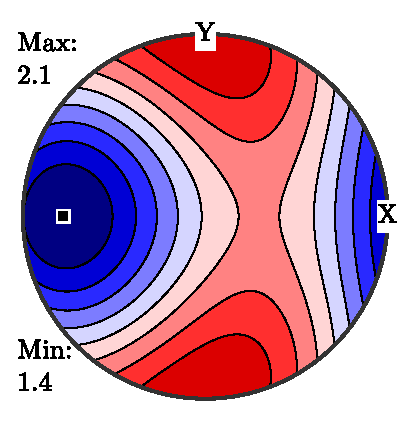
\includegraphics[width=4cm]{pic/sigmaMin}

      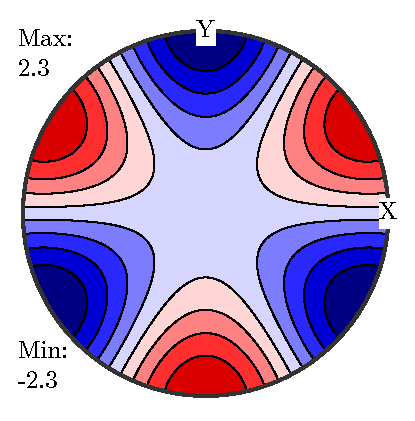
\includegraphics[width=4cm]{pic/piezoComplete}
    \end{column}

  \end{columns}

\end{frame}

\subsection*{Field vs. Matter Tensors}

\begin{frame}[fragile]
  \frametitle{Field Tensors vs. Matter Tensors}

  \begin{overlayarea}{\textwidth}{\textheight}

    \begin{columns}
      \begin{column}{0.7\textwidth}
        \structure{field tensors:}
        \begin{itemize}
        \item in specimen coordinates
        \item describe applied forces like:
          stress, electric field
        \end{itemize}
        \begin{lstlisting}[style=input]
sigma = tensor(M,'name','stress',...
               'unit','MPa');
        \end{lstlisting}

        \pause
        \medskip

        \structure{matter tensors:}
        \begin{itemize}
        \item in crystal coordinates
        \item describe physical properties like: electrical or thermal
          conductivity, magnetic permeability
        \end{itemize}
        \begin{lstlisting}[style=input]
CS = crystalSymmetry('321',...
'mineral','Quartz', 'X||a*', 'Z||c')
P = tensor(M,CS,'name',...
    'piecoelectricity','unit','C/N')
        \end{lstlisting}


      \end{column}
      \begin{column}{0.28\textwidth}
        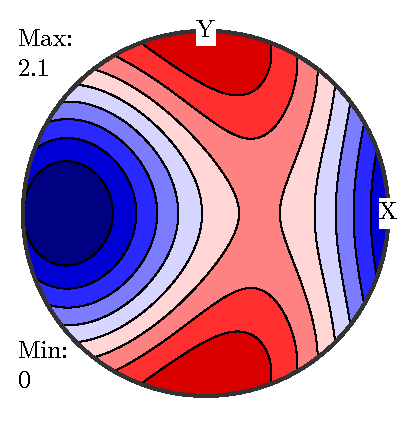
\includegraphics[width=\textwidth]{pic/sigma}

        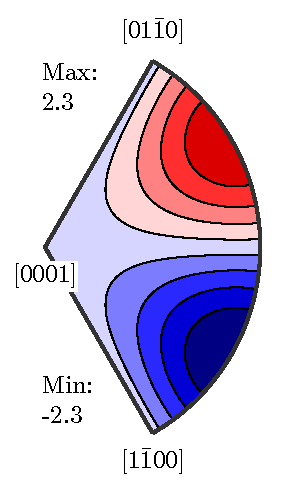
\includegraphics[width=0.7\textwidth]{pic/piezo}
      \end{column}
    \end{columns}



%   \begin{description}
%     \item[field tensors] applied forces, like stress, strain, or a electric
%     field
%     \item[matter tensors] physical properties like electrical or thermal
%     conductivity, magnetic permeability, etc., of a crystalline specimen
%   \end{description}

%   \begin{onlyenv}<2->
%     \begin{lstlisting}[style=input]
% CS = crystalSymmetry('triclinic','mineral','Talc')
% \end{lstlisting}
% \vspace{-0.3cm}
%   \end{onlyenv}

% \begin{onlyenv}<3>
%   \begin{lstlisting}[style=input]
% M = [[219.8  59.6  -4.8 -0.8 -33.8 -1.0];...
%      [ 59.6 216.3  -3.6  1.7 -16.5 -0.6];...
%      [ -4.8  -3.6  48.8  4.1 -15.5 -3.5];...
%      [ -0.8   1.7   4.1 26.5  -3.6 -6.4];...
%      [-33.8 -16.5 -15.5 -3.6  22.8 -1.6];...
%      [ -1.0  -0.6  -3.5 -6.4  -1.6 78.2]];

% C = tensor(M,'name','stiffness','unit','GPa',S)
%   \end{lstlisting}
% \end{onlyenv}
% \begin{onlyenv}<4->
% \begin{lstlisting}[style=input]
% C = tensor(M,'name','stiffness','unit','GPa',S)
% \end{lstlisting}
% \vspace{-0.3cm}
% \end{onlyenv}
% \begin{onlyenv}<4>
% \begin{lstlisting}[style=output]
% C = elastic stiffness /+tensor+/
%      unit: GPa
%      rank: 4 (3 x 3 x 3 x 3)
%   mineral: Talc (triclinic, X||a*, Z||c)

%   tensor in Voigt matrix representation
%   219.83    59.66   -4.82  -0.82  -33.87   -1.04
%    59.66   216.38   -3.67   1.79  -16.51   -0.62
%    -4.82    -3.67   48.89   4.12  -15.52   -3.59
%    -0.82     1.79    4.12  26.54   -3.60   -6.41
%   -33.87   -16.51  -15.52  -3.60   22.85   -1.67
%    -1.04    -0.62   -3.59  -6.41   -1.67   78.29
% \end{lstlisting}
% \end{onlyenv}

% \bigskip

% \begin{onlyenv}<5->
% import a tensor from the \emph{Material Properties Open Database}

% \vspace{-0.2cm}
% \begin{lstlisting}[style=input]
% T = loadTensor('1000055.mpod')
% \end{lstlisting}

% \end{onlyenv}

  \end{overlayarea}


\end{frame}



\section{Average Tensors}
\label{sec:average-tensors}

\subsection*{Rotating Tensors}

\begin{frame}[fragile]
  \frametitle{Rotating Tensors}

  \begin{overlayarea}{\textwidth}{\textheight}
      Consider the piezoelectricity tensor
  \vspace{-0.2cm}
        \begin{lstlisting}[style=input]
P=tensor(M,CS,'name','piecoelectricity','unit','C/N')
\end{lstlisting}
\begin{onlyenv}<1>
          \begin{lstlisting}[style=output]
P = tensor (show methods, plot)
  propertyname    : piecoelectricity
  unit            : C/N
  rank            : 3 (3 x 3 x 3)
  doubleConvention: true
  mineral         : Quartz (321, X||a*, Y||b, Z||c)

  tensor in compact matrix form:
     0     0     0 -0.67     0   4.6
   2.3  -2.3     0     0  0.67     0
     0     0     0     0     0     0
        \end{lstlisting}
      \end{onlyenv}

      \pause
      \medskip
      Remember orientations transforms crystal into specimen coordinates
      \vspace{-0.2cm}
  \begin{lstlisting}[style=input]
ori = orientation('Euler',10*degree,20*degree,0,CS)
rotate(P,ori)
  \end{lstlisting}
\begin{onlyenv}<2>
  \vspace{-.3cm}
\begin{lstlisting}[style=output]
ans = tensor (show methods, plot)
  propertyname    : piecoelectricity
  rank            : 3 (3 x 3 x 3)
  doubleConvention: true

  tensor in compact matrix form:
  -1.08  1.25 -0.17 -0.01  1.47  3.72
   1.92 -1.63 -0.29 -1.29  1.10  1.86
   0.76 -0.66 -0.09 -0.46  0.30  0.43
\end{lstlisting}
\end{onlyenv}

\pause
\medskip

Contrary, an inverse orientation transforms specimen coordinates into crystal
coordinates.
\vspace{-0.2cm}
  \begin{lstlisting}[style=input]
rotate(sigma,inv(ori))
  \end{lstlisting}
\begin{onlyenv}<3>
  \vspace{-.3cm}
  \begin{lstlisting}[style=output]
ans = stress tensor (show methods, plot)
  unit   : MPa
  rank   : 2 (3 x 3)
  mineral: Quartz (321, X||a*, Y||b, Z||c)

  1.47  0.17  0.14
  0.17  2.03 -0.12
  0.14 -0.12  1.85
\end{lstlisting}
\end{onlyenv}
\end{overlayarea}
\end{frame}

\subsection*{Avarage Tensors}

\begin{frame}[fragile]
  \frametitle{Average Tensors}

  The average tensorial property of a specimen is the mean of matter tensors
  rotated according to each grain orientation $o_{m}$, $m=1,\ldots,M$.

\medskip
\pause

The Voigt and the Reuss averages of a tensor $T$ are defines as
\begin{equation*}
  \left<T\right>^{\text{Voigt}}
  = \sum_{m=1}^{M} V_{m} T(o_{m}), \quad
  \left<T\right>^{\text{Reuss}}
  = \left[ \sum_{m=1}^{M} V_{m} T^{-1}(o_{m}) \right]^{-1}.
\end{equation*}

\medskip
\pause

For EBSD data this is computed by
\begin{lstlisting}[style=input]
[TVoigt, TReus, THill] = calcTensor(ebsd,T)
\end{lstlisting}

\medskip
\pause

and for an ODF by
\begin{lstlisting}[style=input]
[TVoigt, TReus, THill] = calcTensor(odf,T)
\end{lstlisting}

\end{frame}

\section{Elastic Deformation}
\label{sec:elasticity}

\subsection*{basics}

\begin{frame}[fragile]
  \frametitle{Elastic Deformation}

  \begin{columns}
    \begin{column}{0.65\textwidth}
      \begin{overlayarea}{\textwidth}{\textheight}
        Imort some stiffness tensor
        \vspace{-0.2cm}
      \begin{lstlisting}[style=input]
cs = loadCIF('Nickel')
C = loadTensor('IN739LC.GPa',...
    cs,'name','elastic stiffness')
\end{lstlisting}
\begin{onlyenv}<1>
  \vspace{-0.3cm}
  \begin{lstlisting}[style=output]
C = /+elastic stiffness tensor+/ (show methods)
  unit   : GPa
  rank   : 4 (3 x 3 x 3 x 3)
  mineral: Ni (432)

  tensor in Voigt matrix representation:
 235.16 147.67 147.67      0      0      0
 147.67 235.16 147.67      0      0      0
 147.67 147.67 235.16      0      0      0
      0      0      0 122.53      0      0
      0      0      0      0 122.53      0
      0      0      0      0      0 122.53
  \end{lstlisting}
\end{onlyenv}

\pause

The inverse of the stiffness is the compliance
\vspace{-0.2cm}
\begin{lstlisting}[style=input]
S = inv(C)
\end{lstlisting}

\begin{onlyenv}<2>
  \vspace{-0.3cm}
  \begin{lstlisting}[style=output]
S = /+elastic compliance tensor+/
  unit            : 1 / GPa
  rank            : 4 (3 x 3 x 3 x 3)
  doubleConvention: true
  mineral         : Ni (432)

  tensor in Voigt matrix represent.: *10^-4
  82.48 -31.82 -31.82      0      0      0
 -31.82  82.48 -31.82      0      0      0
 -31.82 -31.82  82.48      0      0      0
      0      0      0  81.61      0      0
      0      0      0      0  81.61      0
      0      0      0      0      0  81.61
  \end{lstlisting}
  \end{onlyenv}

  \pause

  Consider unaxial stress $\sigma$
  \vspace{-0.2cm}
  \begin{lstlisting}[style=input]
sigma = tensor(M,'name','stress')
\end{lstlisting}
\begin{onlyenv}<3>
    \vspace{-0.4cm}
  \begin{lstlisting}[style=output]
sigma = /+stress tensor+/ (show methods, plot)
  rank: 2 (3 x 3)

 0 0 0
 0 0 0
 0 0 1
  \end{lstlisting}
  \end{onlyenv}

  \pause

  strain $\varepsilon_{ij} = S_{klij} \sigma_{kl}$
  \vspace{-0.2cm}
  \begin{lstlisting}[style=input]
eps = EinsteinSum(rotate(S,ori),...
    [-1 -2 1 2],sigma,[-1 -2])
\end{lstlisting}
  \vspace{-0.4cm}
  \begin{lstlisting}[style=output]
eps = /+strain tensor+/ (show methods, plot)
  rank: 2 (3 x 3)

 147.67      0      0
      0 147.67      0
      0      0 235.16
  \end{lstlisting}
\end{overlayarea}
\end{column}

    \begin{column}{0.35\textwidth}
      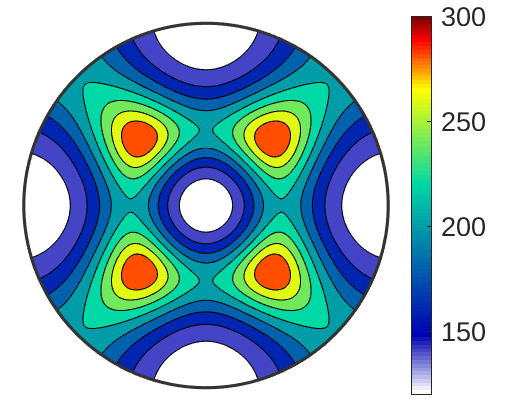
\includegraphics[width=\textwidth]{pic/Nickel_SC_2d.pdf}

      \includegraphics[width=\textwidth]{pic/Nickel_SC_3d.pdf}
    \end{column}
  \end{columns}

\end{frame}



\subsection*{Elasticity Tensors}

\begin{frame}[fragile]
  \frametitle{Elasticity Tensors}

  \vspace{-0.5cm}
  \begin{overlayarea}{\textwidth}{\textheight}

  \begin{columns}
    \begin{column}{7.7cm}

      derived elastic properties
      \vspace{-0.2cm}
\begin{lstlisting}[style=input]
beta = volumeCompressibility(C)
beta = linearCompressibility(C,x)
E    = YoungsModulus(C,x)
G    = shearModulus(C,h,u)
nu   = PoissonRatio(C,x,y)
T    = ChristoffelTensor(C,n)
\end{lstlisting}

\pause

\vspace{-0.2cm}
\begin{lstlisting}[style=input]
nu = C.PoissonRatio([],xvector);
contourf(nu,'minmax')
mtexColorMap blue2red
\end{lstlisting}

\pause

\vspace{-0.2cm}
\begin{lstlisting}[style=input]
[value,pos] = max(nu)
\end{lstlisting}

\begin{onlyenv}<3>
  \vspace{-0.3cm}
  \begin{lstlisting}[style=output]
value =
    0.6956
pos = /+vector3d+/
 size: 1 x 1
          x         y         z
  -0.918733         0  0.394879
  \end{lstlisting}
\end{onlyenv}

\pause

\vspace{-0.2cm}
\begin{lstlisting}[style=input]
annotate(pos,'label','max')
\end{lstlisting}


    \end{column}
    \begin{column}{4cm}
      \only<2-3>{
        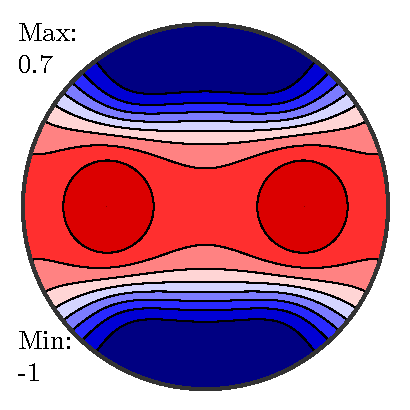
\includegraphics[width=4cm]{pic/PRa}}
      \only<4>{
        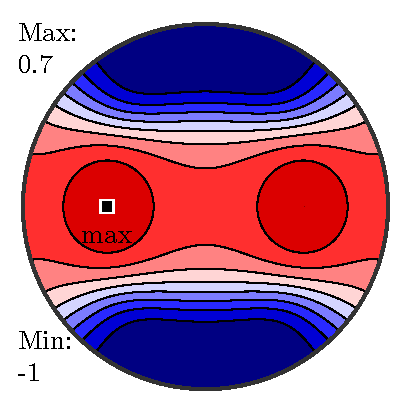
\includegraphics[width=4cm]{pic/PRb}}
    \end{column}
  \end{columns}
\end{overlayarea}

\end{frame}



\subsection*{evolution}

\begin{frame}[fragile]
  \frametitle{Evolution of Elasticity}

  \vspace{-0.3cm}
  \begin{overlayarea}{\textwidth}{\textheight}

    \begin{onlyenv}<1->
      \vspace{-0.3cm}
      \begin{lstlisting}[style=input]
for k = 1:5
  odf{k} = BinghamODF([-10,-10,5*k-15,10],cs);
end
\end{lstlisting}
    \end{onlyenv}
    \begin{onlyenv}<1>
      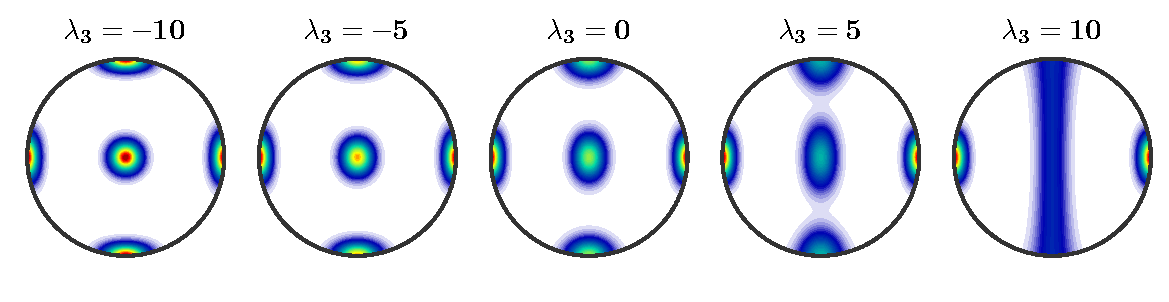
\includegraphics[width=\textwidth]{pic/binghamPDF.pdf}
    \end{onlyenv}

    \begin{onlyenv}<2>
      \vspace{-0.3cm}
\begin{lstlisting}[style=input]
for k = 1:length(odf)
  [C_v,C_r] = calcTensor(odf{k},C);
  psr_v(k) = C_v.YoungsModulus(vector3d.Z);
  psr_r(k) = C_r.YoungsModulus(vector3d.Z);
end
\end{lstlisting}
    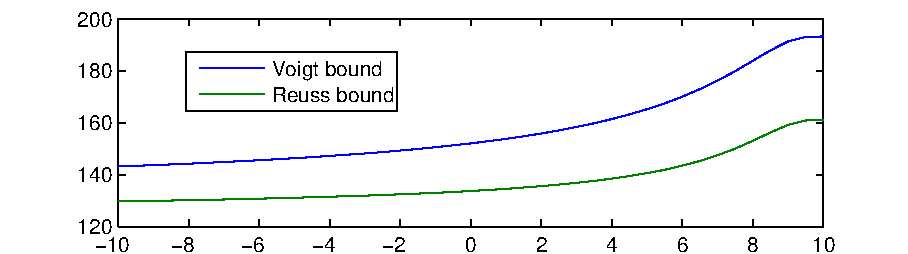
\includegraphics[width=\textwidth]{pic/VR.pdf}
    \end{onlyenv}
  \end{overlayarea}
\end{frame}

\subsection*{Wave Velocities}

\begin{frame}[fragile]
  \frametitle{Wave Velocities}

\begin{lstlisting}[style=input]
[vp,vs1,vs2,pp,ps1,ps2] = velocity(C,[],rho)
\end{lstlisting}

  \begin{columns}
  \begin{column}{8.5cm}

\begin{lstlisting}[style=input]
plot(vp,'minmax')

hold on
plot(pp)
hold off
\end{lstlisting}

\bigskip
\pause

    \begin{lstlisting}[style=input]
plot(vs1-vs2,'minmax')

hold on
plot(ps1)
hold off
\end{lstlisting}

  \end{column}
    \begin{column}{3.5cm}
      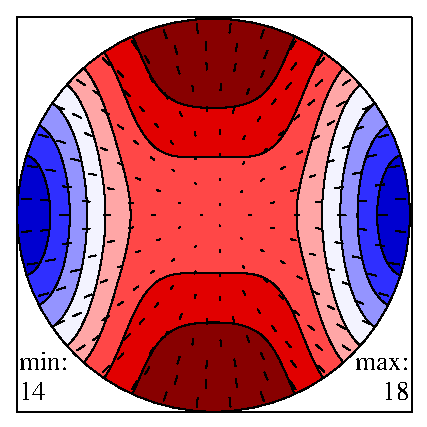
\includegraphics[width=3.5cm]{pic/vp-pp}

      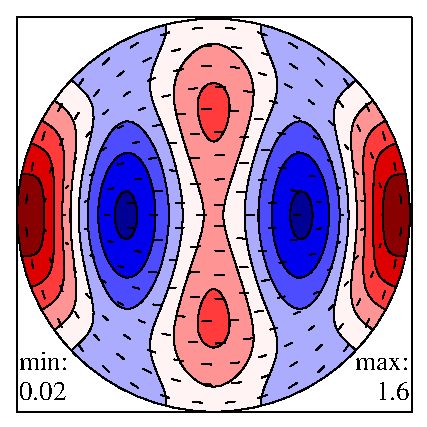
\includegraphics[width=3.5cm]{pic/vs12-ps1}
  \end{column}

  \end{columns}

\end{frame}

\section{Plastic Deformation}
\label{sec:plastic-deformation}

\subsection*{Schmidt Factor}

\begin{frame}[fragile]
  \frametitle{Schmidt Factor}

  Consider the slip system
  \begin{lstlisting}[style=input]
d = Miller(0,-1,1,cs,'uvw');  % slip direction
n = Miller(1,1,1,cs,'hkl');   % slip plane normal
\end{lstlisting}

\pause

and the extension direction
  \begin{lstlisting}[style=input]
r = vector3d(0,0,1)           % extension direction
\end{lstlisting}

\pause

\medskip

Then the Schmid factor in direction $\mathbf r$ is given by
\begin{equation*}
  SF = \cos \theta \cos \rho
\end{equation*}

\pause

In \MTEX this can be computed by
  \begin{lstlisting}[style=input]
SF = dot(n,r) * dot(b,r)
  \end{lstlisting}

\end{frame}

\subsection*{slip systems}

\begin{frame}[fragile]
  \frametitle{Slip Systems}

  \begin{columns}
    \begin{column}{8cm}
      \vspace{-0.6cm}
      \begin{overlayarea}{\textwidth}{8cm}
  \begin{lstlisting}[style=input]
sS = slipSystem(d,n)
\end{lstlisting}
\begin{onlyenv}<1>
  \vspace{-0.3cm}
  \begin{lstlisting}[style=output]
sS = /+slipSystem+/
 symmetry: 432
 CRSS: 1
 size: 1 x 1
  u   v   w | h   k   l
  0  -1   1   1   1   1
  \end{lstlisting}
\end{onlyenv}

\pause

      \vspace{-0.1cm}
  \begin{lstlisting}[style=input]
sS = slipSystem.fcc(cs)
\end{lstlisting}
\begin{onlyenv}<2>
  \vspace{-0.3cm}
  \begin{lstlisting}[style=output]
sS = /+slipSystem+/
 symmetry: 432
 CRSS: 1
 size: 1 x 1
  u   v   w | h   k   l
  0   1  -1   1   1   1
  \end{lstlisting}
\end{onlyenv}

\pause
      \vspace{-0.1cm}
        \begin{lstlisting}[style=input]
sS.symmetrise('antipodal')
        \end{lstlisting}
        \begin{onlyenv}<3>
          \vspace{-0.3cm}
          \begin{lstlisting}[style=output]
sS = /+slipSystem+/
 symmetry: 432
 CRSS: 1
 size: 12 x 1
   u   v   w | h   k   l
   0  -1   1   1   1   1
   1   0  -1   1   1   1
  -1   1   0   1   1   1
  -1   1   0   1   1  -1
  -1   0  -1   1   1  -1
   0  -1  -1   1   1  -1
   0  -1   1  -1   1   1
  -1   0  -1  -1   1   1
  -1  -1   0  -1   1   1
   1   0  -1   1  -1   1
  -1  -1   0   1  -1   1
   0  -1  -1   1  -1   1
          \end{lstlisting}
        \end{onlyenv}

        \pause

        \vspace{-0.1cm}
  \begin{lstlisting}[style=input]
sS.SchmidFactor(vector3d.Z)
\end{lstlisting}

\pause

\vspace{-0.1cm}
\begin{lstlisting}[style=input]
plot(sS.SchmidFactor)
\end{lstlisting}

\pause

\vspace{-0.1cm}
\begin{lstlisting}[style=input]
sigma=tensor([1 0 1;0 0 0;1 0 1],...
  'name','stress')
sS.SchmidFactor(sigma)
\end{lstlisting}


\end{overlayarea}
\end{column}
\begin{column}{4cm}
  \only<4->{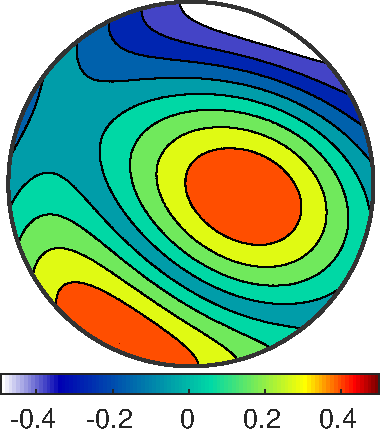
\includegraphics[width=\textwidth]{pic/sFsingle}}
\end{column}
\end{columns}



\end{frame}


\subsection*{symmetric slipsystems}

\begin{frame}[fragile]
  \frametitle{Critical Resolved Shear Stress}

  \begin{columns}
    \begin{column}{8cm}
      \begin{overlayarea}{\textwidth}{8cm}

the Schmid factor for a list of tension directions
\vspace{-0.2cm}
\begin{lstlisting}[style=input]
sS = sS.symmetrise('antipodal')
r = plotS2Grid('upper')
SF = sS.SchmidFactor(r)
  \end{lstlisting}

\pause
\vspace{0.1cm}
take the maximum Schmidfactor
\vspace{-0.2cm}
  \begin{lstlisting}[style=input]
[maxSF,id] = max(abs(SF),[],2)
contourf(r,maxSF)
  \end{lstlisting}

\pause

\vspace{0.1cm}
the active slip system
\vspace{-0.2cm}
\begin{lstlisting}[style=input]
contourf(r,id,'contours',12)
hold on
quiver(r,sS(id).n,'Color','r');
quiver(r,sS(id).b,'Color','g');
hold off

\end{lstlisting}
\end{overlayarea}
\end{column}
\begin{column}{4cm}

  \begin{overlayarea}{\textwidth}{8cm}
    \only<2->{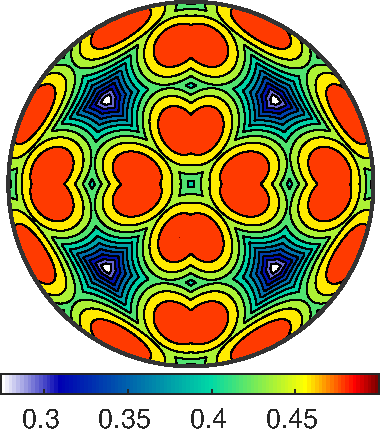
\includegraphics[width=\textwidth]{pic/sFsym}}

    \vspace{-0.2cm}

    \only<3->{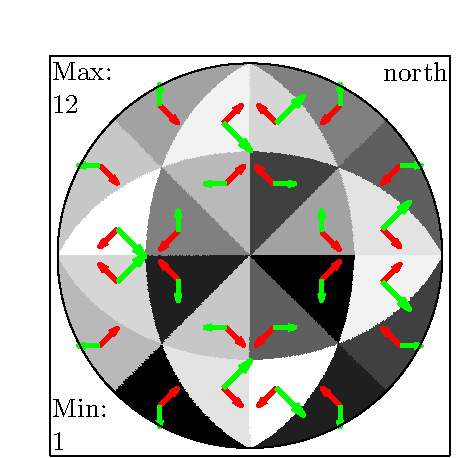
\includegraphics[height=3.5cm]{pic/SFActive}}
  \end{overlayarea}

\end{column}
\end{columns}

\end{frame}

\subsection*{The Schmid Factor for Grains}

\begin{frame}[fragile]
  \frametitle{The Schmid Factor for Grains}
  \vspace{-0.5cm}
  \begin{overlayarea}{\textwidth}{\textheight}
    \begin{onlyenv}<1->
\begin{lstlisting}[style=input]
sigma = tensor([[0 0 0];[0 0 0];[0 0 1]],'stress')
\end{lstlisting}
  \end{onlyenv}
  \begin{onlyenv}<1>
\begin{lstlisting}[style=output]
sigma = stress /+tensor+/ (show methods, plot)
  rank: 2 (3 x 3)

 0 0 0
 0 0 0
 0 0 1
\end{lstlisting}
    \end{onlyenv}
    \vspace{-0.3cm}
    \begin{onlyenv}<2->
\begin{lstlisting}[style=input]
sigmaCS = rotate(sigma,inv(grains.meanOrientation))
\end{lstlisting}
    \end{onlyenv}
    \begin{onlyenv}<2>
\begin{lstlisting}[style=output]
sigmaCS = stress /+tensor+/ (show methods, plot)
  size   : 465 x 1
  rank   : 2 (3 x 3)
  mineral: iron (m-3m)
\end{lstlisting}
    \end{onlyenv}
    \begin{onlyenv}<3->
      \vspace{-0.3cm}
      \begin{lstlisting}[style=input]
SF = sS.SchmidFactor(sigmaCS);
[maxSF,active] = max(abs(SF),[],2);
\end{lstlisting}
    \end{onlyenv}
    \begin{onlyenv}<4>
      \vspace{-0.3cm}
\begin{lstlisting}[style=input]
plot(grains,maxSF)
\end{lstlisting}
    \end{onlyenv}
    \begin{onlyenv}<5->
      \vspace{-0.3cm}
\begin{lstlisting}[style=input]
for id = unique(active)
  plot(grains(active==id),'FaceColor',color{id},...
  'DisplayName',[char(nSym(id)) ' ' char(bSym(id))])
end
\end{lstlisting}

\end{onlyenv}
    \begin{onlyenv}<4>
      \centerline{
        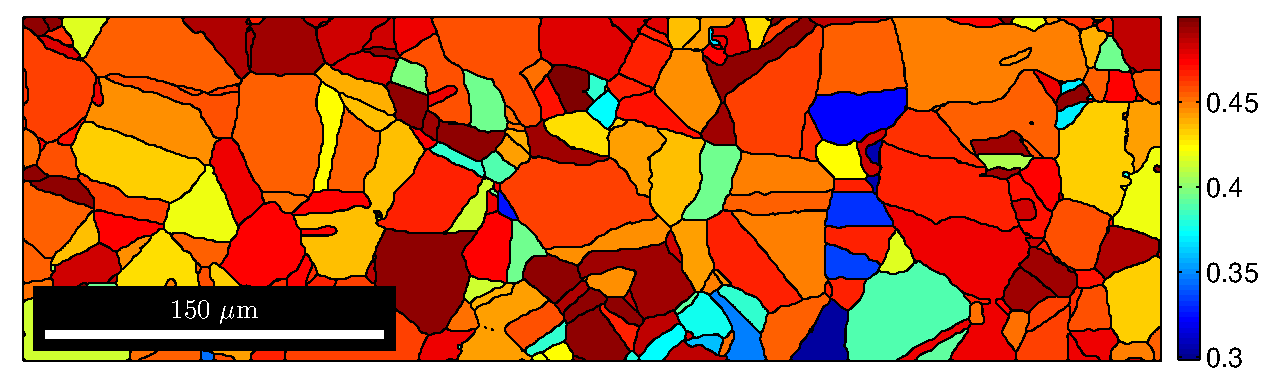
\includegraphics[width=\textwidth]{pic/shearStress.pdf}}
    \end{onlyenv}
    \begin{onlyenv}<5> \centerline{
        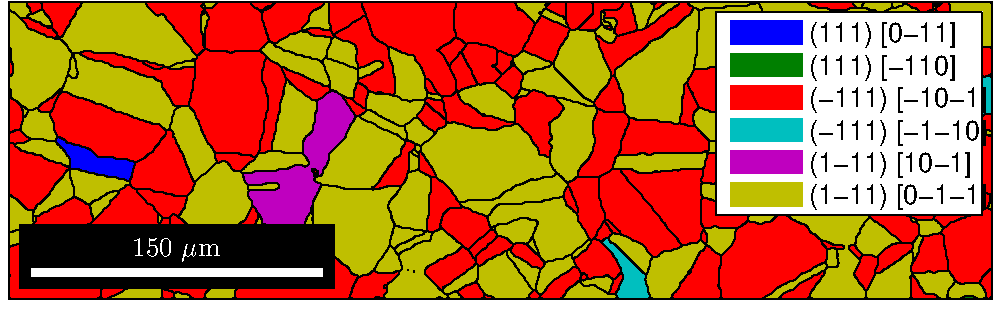
\includegraphics[width=0.9\textwidth]{pic/slipSystem.pdf}}
    \end{onlyenv}

 \end{overlayarea}
\end{frame}

\subsection*{Plastic deformation - stress based analysis}

\begin{frame}[fragile]
  \frametitle{Plastic deformation - stress based analysis}

convert slip systems to specimen coordinates:
\vspace{-0.2cm}
\begin{lstlisting}[style=input]
ori = grains.meanOrientation;
sSGrains =  ori * sS
\end{lstlisting}
      \begin{onlyenv}<1>
        \vspace{-0.2cm}
      \begin{lstlisting}[style=output]
sSGrains = /+slipSystem+/ (show methods, plot)
 size: 37 x 12
      \end{lstlisting}
    \end{onlyenv}

\pause
\begin{columns}
  \begin{column}{0.65\textwidth}

some uniaxial stress:
\vspace{-0.2cm}
  \begin{lstlisting}[style=input]
sigma = tensor.diag([1,0,0])
\end{lstlisting}
      \begin{onlyenv}<2>
        \vspace{-0.2cm}
        \begin{lstlisting}[style=output]
sigma = /+tensor+/ (show methods, plot)
  rank: 2 (3 x 3)

 1 0 0
 0 0 0
 0 0 0
      \end{lstlisting}
    \end{onlyenv}

\pause

the Schmid Factor for each slip system:
\vspace{-0.2cm}
\begin{lstlisting}[style=input]
SF = sSGrains.SchmidFactor(sigma)
\end{lstlisting}

\pause

determine for each grain the active slip system
\vspace{-0.2cm}
\begin{lstlisting}[style=input]
[maxSF,active] = max(SF,[],2);
plot(grains,maxSF)
\end{lstlisting}

\pause

plot slip direction and slip plane
\vspace{-0.2cm}
\begin{lstlisting}[style=input]
sSActive = ori .* sS(active)
quiver(grains,sSActive.b)
quiver(grains,sSActive.n)
\end{lstlisting}

\end{column}
\begin{column}{0.35\textwidth}
  \only<4>{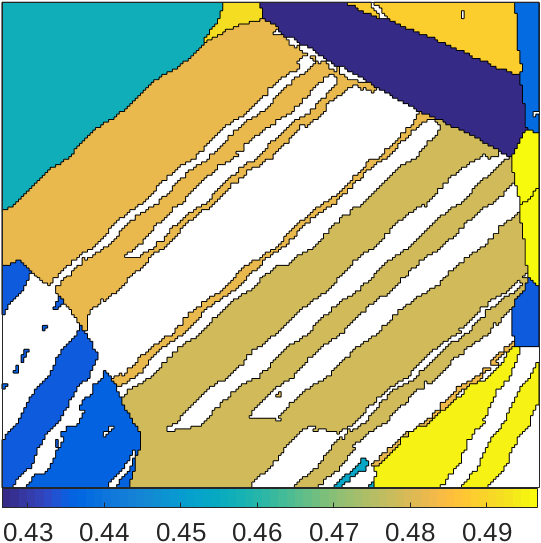
\includegraphics[width=\textwidth]{pic/SF.png}}
  \only<5>{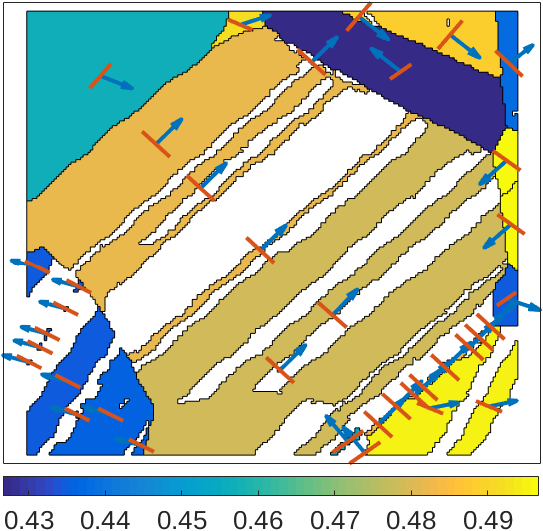
\includegraphics[width=\textwidth]{pic/SFSlip.png}}
\end{column}
\end{columns}

\end{frame}

\subsection*{strain based analysis}

\begin{frame}[fragile]
  \frametitle{Plastic deformation - strain based analysis}

some strain:
\vspace{-0.2cm}
      \begin{lstlisting}[style=input]
q = 0.25; eps = tensor.diag([1 -q -(1-q)])
      \end{lstlisting}
      \begin{onlyenv}<1>
        \vspace{-0.2cm}
        \begin{lstlisting}[style=output]
eps = /+tensor+/ (show methods, plot)
  rank: 2 (3 x 3)
  rank: 2 (3 x 3)

     1     0     0
     0 -0.25     0
     0     0 -0.75
   \end{lstlisting}
    \end{onlyenv}

\pause

    transform strain to crystal coordinates
    \vspace{-0.2cm}
      \begin{lstlisting}[style=input]
ori = grains('fcc').meanOrientation
epsGrain = inv(ori) * eps
      \end{lstlisting}
      \begin{onlyenv}<2>
        \vspace{-0.2cm}
        \begin{lstlisting}[style=output]
epsGrain = /+tensor+/ (show methods, plot)
  size   : 37 x 1
  rank   : 2 (3 x 3)
  mineral: Austenite (fcc, 432)
        \end{lstlisting}
      \end{onlyenv}

      \pause

compute Taylor factor
      \vspace{-0.2cm}
\begin{lstlisting}[style=input]
[M,b,mori] = calcTaylor(epsGrain,sS);
\end{lstlisting}

  \begin{columns}
    \begin{column}{0.62\textwidth}

        \vspace{-0.5cm}
\begin{lstlisting}[style=input]
plot(grains,M)
      \end{lstlisting}

      \pause

      \begin{lstlisting}[style=input]
[bMax,bMaxId] = max(b,[],2);
sSGrains = ori .* sS(bMaxId);
hold on
quiver(grains,sSGrains.b)
quiver(grains,sSGrains.n)
hold off
\end{lstlisting}


    \end{column}
     \begin{column}{0.35\textwidth}
       \only<3>{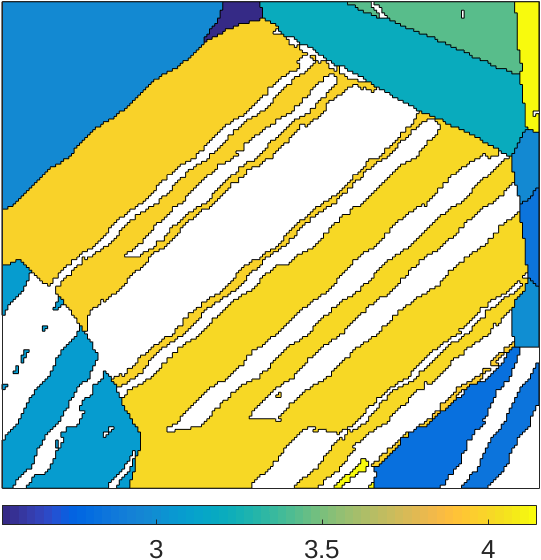
\includegraphics[width=\textwidth]{pic/taylor.png}}
       \only<4>{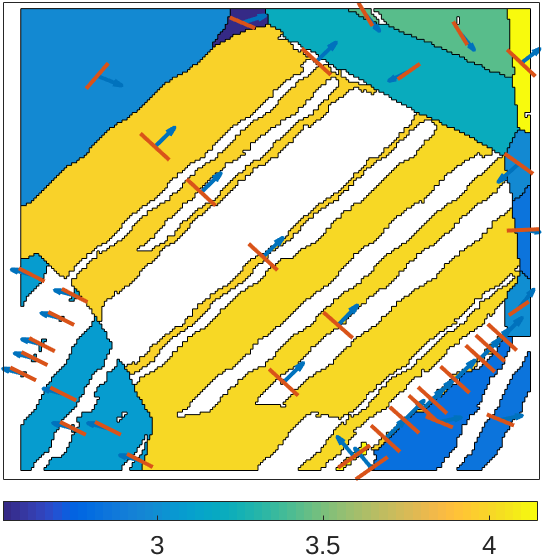
\includegraphics[width=\textwidth]{pic/taylorSlip.png}}
     \end{column}
   \end{columns}
%   \end{overlayarea}
\end{frame}

\subsection*{Rolling texture evolution}

\begin{frame}[fragile]
  \frametitle{Rolling texture evolution}

  \begin{columns}
    \begin{column}{0.7\textwidth}

      \vspace{-0.7cm}
      \begin{overlayarea}{\textwidth}{8cm}

\begin{lstlisting}[style=input]
ori = orientation.rand(10000,CS_Aus)
h = Miller({0,0,1},{1,1,1}),CS_Aus)
plotPDF(ori,'contourf')
\end{lstlisting}

\pause

the slip systems
\vspace{-0.2cm}
        \begin{lstlisting}[style=input]
sS=symmetrise(slipSystem.fcc(CS_Aus))
      \end{lstlisting}

      \begin{onlyenv}<2>
        \vspace{-0.2cm}
      \begin{lstlisting}[style=output]
sS = /+slipSystem+/ (show methods, plot)
 size: 12 x 1
 mineral: Austenite (fcc) (432)
   u   v   w | h   k   l
   0   1  -1   1   1   1
  -1   0   1   1   1   1
   1  -1   0   1   1   1
   1  -1   0   1   1  -1
   1   0   1   1   1  -1
   0   1   1   1   1  -1
   0   1  -1  -1   1   1
   1   0   1  -1   1   1
   1   1   0  -1   1   1
  -1   0   1   1  -1   1
   1   1   0   1  -1   1
   0   1   1   1  -1   1
      \end{lstlisting}
    \end{onlyenv}

    \pause

30 percent strain
\vspace{-0.2cm}
\begin{lstlisting}[style=input]
q = 0;
eps = 0.3*tensor.diag([1 -q -(1-q)])
\end{lstlisting}

\pause

iterate deformation:
\vspace{-0.2cm}
      \begin{lstlisting}[style=input]
for i = 1:10
  [M,~,mori] =  calcTaylor(...
    inv(ori) * eps ./ 10, sS);
  ori = ori .* mori;
  plotPDF(ori,h,'contourf')
end
\end{lstlisting}

\end{overlayarea}
\end{column}
    \begin{column}{0.29\textwidth}
      \vspace{-1cm}
      \begin{onlyenv}<1-3>
        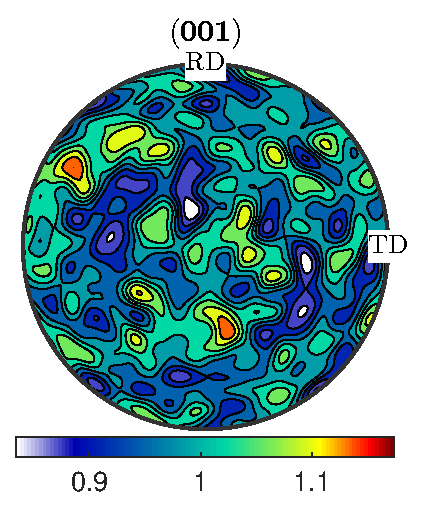
\includegraphics[width=\textwidth]{pic/rolling001}

      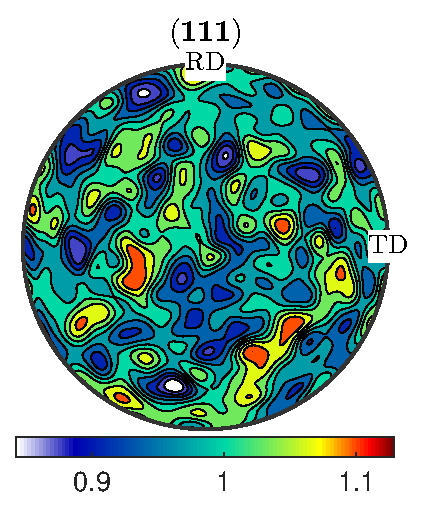
\includegraphics[width=\textwidth]{pic/rolling111}
    \end{onlyenv}

      \begin{onlyenv}<4>
        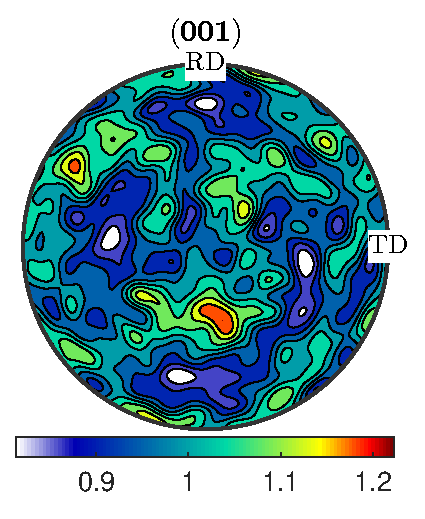
\includegraphics[width=\textwidth]{pic/rolling001_1}

      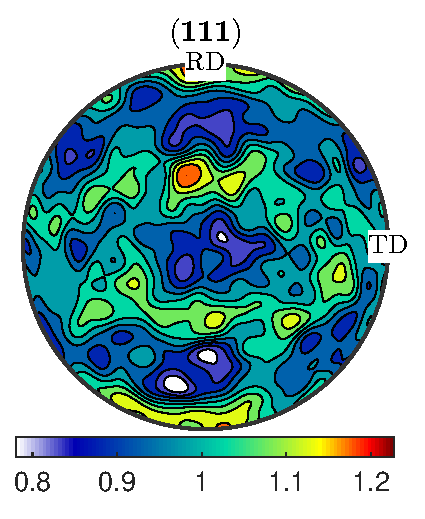
\includegraphics[width=\textwidth]{pic/rolling111_1}
    \end{onlyenv}

    \begin{onlyenv}<5>
        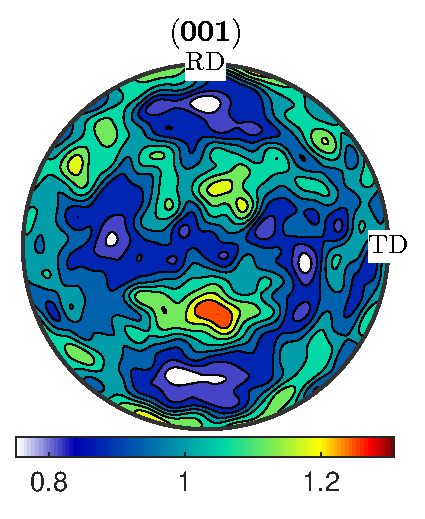
\includegraphics[width=\textwidth]{pic/rolling001_2}

      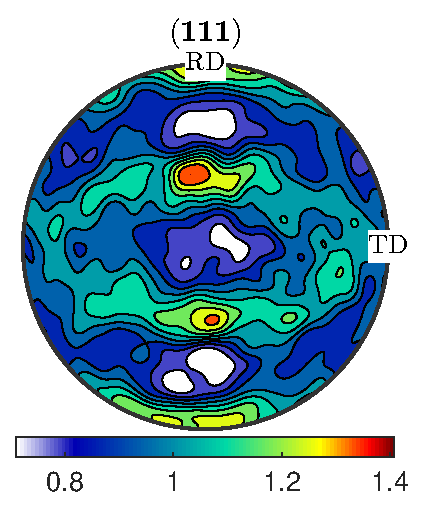
\includegraphics[width=\textwidth]{pic/rolling111_2}
    \end{onlyenv}

        \begin{onlyenv}<6>
        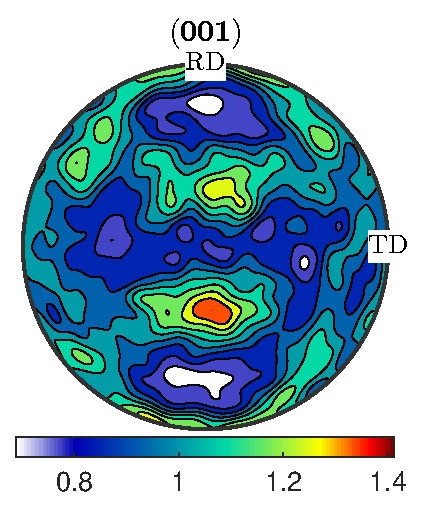
\includegraphics[width=\textwidth]{pic/rolling001_3}

      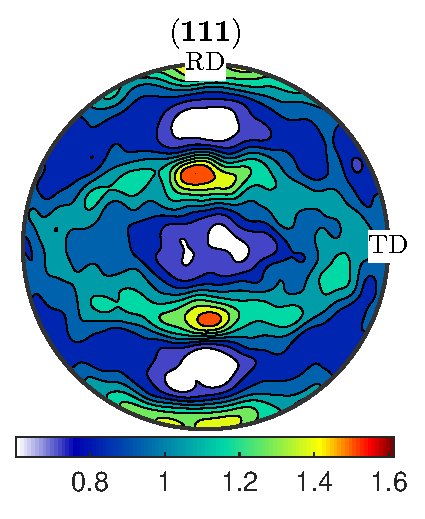
\includegraphics[width=\textwidth]{pic/rolling111_3}
    \end{onlyenv}

            \begin{onlyenv}<7>
        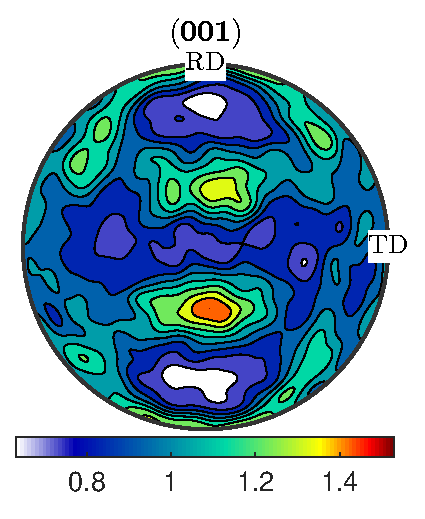
\includegraphics[width=\textwidth]{pic/rolling001_4}

      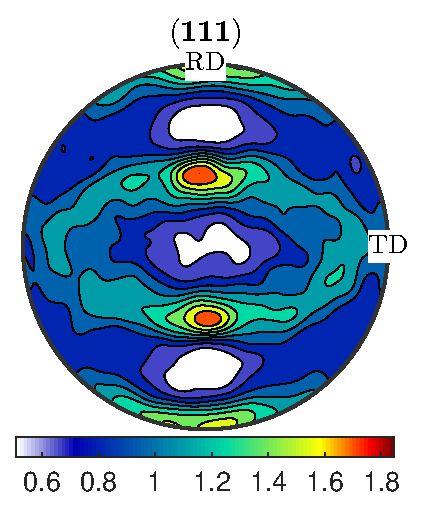
\includegraphics[width=\textwidth]{pic/rolling111_4}
    \end{onlyenv}

                \begin{onlyenv}<8>
        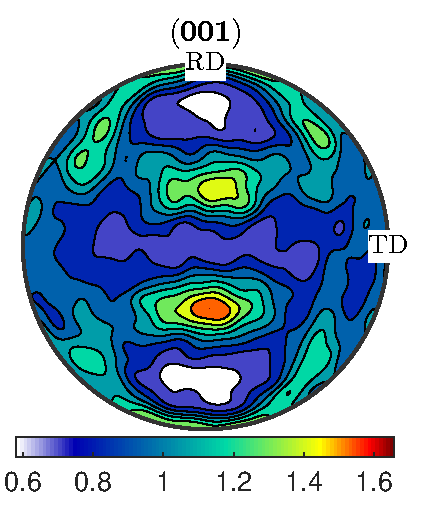
\includegraphics[width=\textwidth]{pic/rolling001_5}

      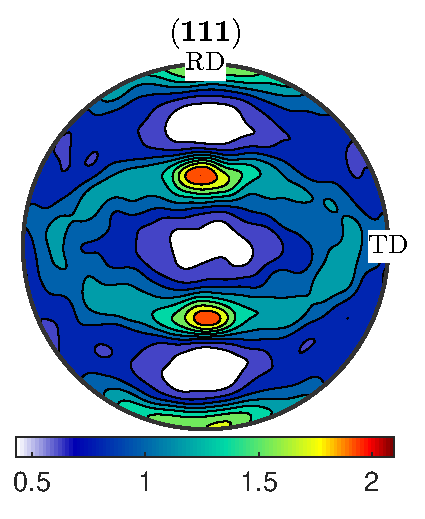
\includegraphics[width=\textwidth]{pic/rolling111_5}
    \end{onlyenv}

                    \begin{onlyenv}<9>
        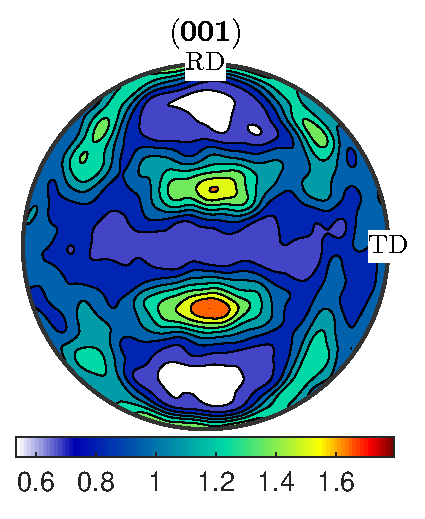
\includegraphics[width=\textwidth]{pic/rolling001_6}

      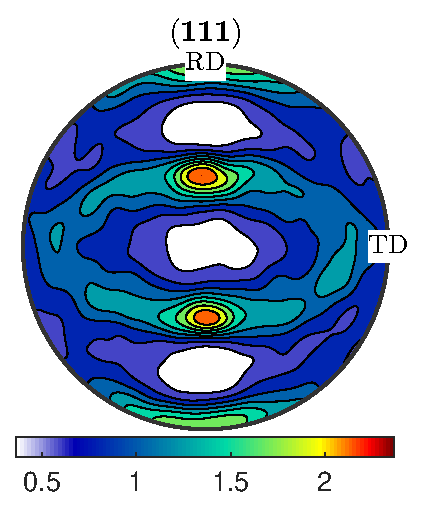
\includegraphics[width=\textwidth]{pic/rolling111_6}
    \end{onlyenv}

                        \begin{onlyenv}<10>
        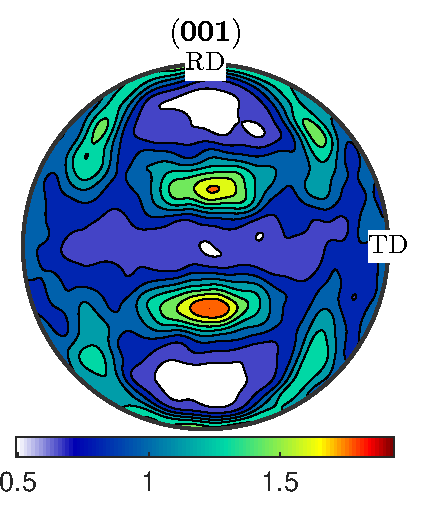
\includegraphics[width=\textwidth]{pic/rolling001_7}

      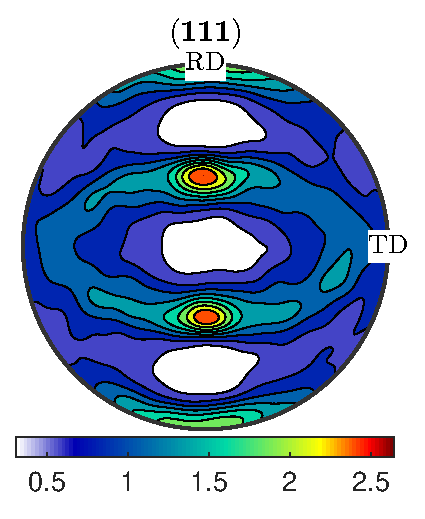
\includegraphics[width=\textwidth]{pic/rolling111_7}
    \end{onlyenv}

                        \begin{onlyenv}<11>
        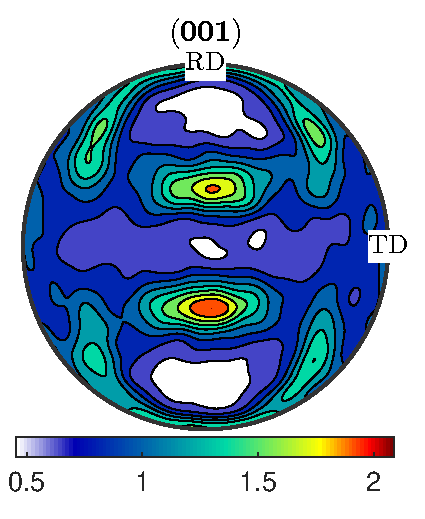
\includegraphics[width=\textwidth]{pic/rolling001_8}

      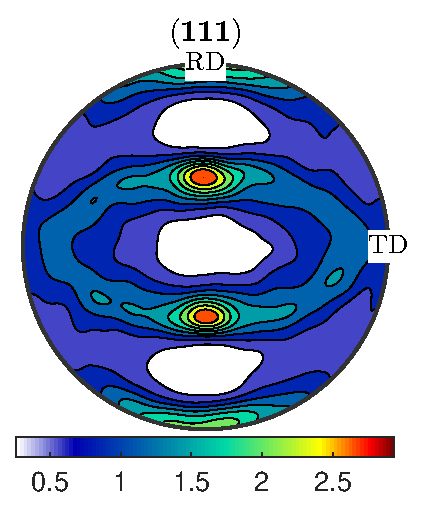
\includegraphics[width=\textwidth]{pic/rolling111_8}
    \end{onlyenv}

                        \begin{onlyenv}<12>
        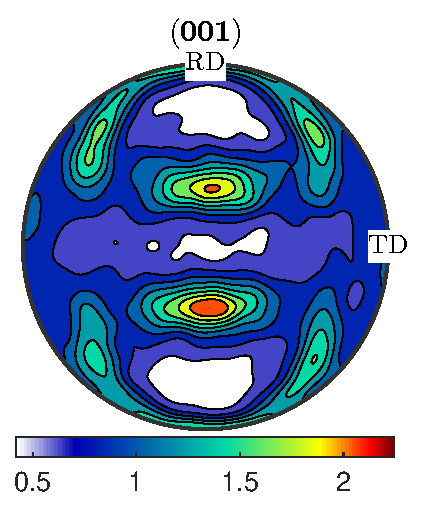
\includegraphics[width=\textwidth]{pic/rolling001_9}

      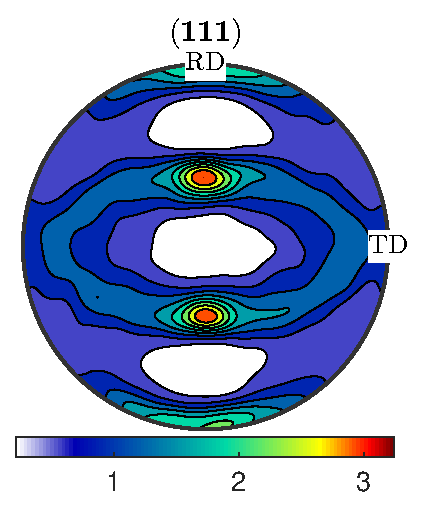
\includegraphics[width=\textwidth]{pic/rolling111_9}
    \end{onlyenv}

                        \begin{onlyenv}<13>
        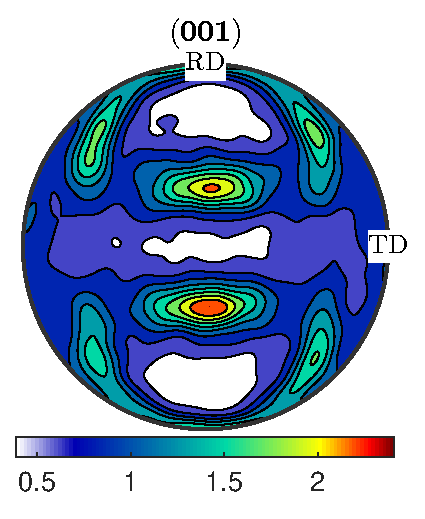
\includegraphics[width=\textwidth]{pic/rolling001_10}

      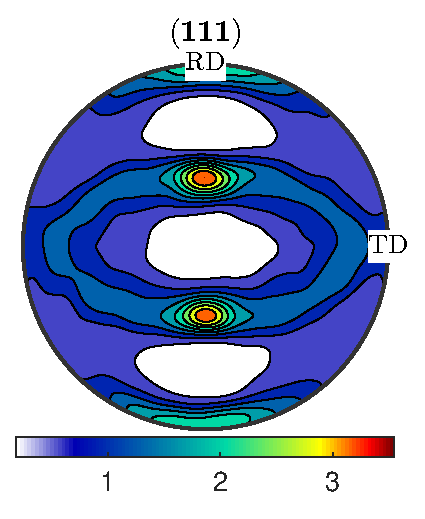
\includegraphics[width=\textwidth]{pic/rolling111_10}
    \end{onlyenv}

  \end{column}
   \end{columns}
%   \end{overlayarea}
\end{frame}

\subsection*{Misc}

\begin{frame}[fragile]
  \frametitle{Misc}
  \vspace{-0.5cm}
  \begin{overlayarea}{\textwidth}{8cm}

      \begin{lstlisting}[style=input]
epsGrain
\end{lstlisting}
\begin{onlyenv}<1>
    \vspace{-0.3cm}
  \begin{lstlisting}[style=output]
epsGrain = strain tensor (show methods, plot)
  size   : 37 x 1
  rank   : 2 (3 x 3)
  mineral: fcc (432)
\end{lstlisting}
\end{onlyenv}
\pause

  \begin{lstlisting}[style=input]
epsGrain(1)
\end{lstlisting}
\begin{onlyenv}<2>
    \vspace{-0.3cm}
    \begin{lstlisting}[style=output]
ans = strain tensor (show methods, plot)
  rank   : 2 (3 x 3)
  mineral: fcc (432)

 *10^-2
  57.35  -24.9 -70.07
  -24.9 -20.11   7.41
 -70.07   7.41 -37.24
\end{lstlisting}
\end{onlyenv}
\pause
\begin{lstlisting}[style=input]
epsGrain{1,1}
\end{lstlisting}
\begin{onlyenv}<3>
  \vspace{-0.3cm}
\begin{lstlisting}[style=output]
ans =
    0.5735
    0.7898
   -0.2335
    0.5767
    0.1689
    0.1850
    0.7818
   -0.1903
   -0.2332
    0.6518
    0.1988
    0.2005
    0.1999
   -0.2329
    0.6348
   -0.2345
    0.1990
   -0.2349
    0.1993
\end{lstlisting}
\end{onlyenv}
\end{overlayarea}
\end{frame}



% % The above procedure may also be applied to grains which has the advantage
% % to be much less computational demanding for large data sets.
% %
% % compute grains
% grains = calcGrains(ebsd)

% % extract the orientations
% ori = get(grains('Fe'),'orientation');

% % transform the stress tensor from specimen to crystal coordinates
% sigmaCS = rotate(sigma001,inv(ori))

% % compute maximum Schmid factor and active slip system
% [Schmid_Max,bActive,nActive,tau,ind] = calcShearStress(sigmaCS,n,b,'symmetrise');

% plot(grains('Fe'),'property',Schmid_Max)
% colorbar



% \begin{frame}
%



% % we observe that the Schmid factor is always between -0.5 and 0.5.
% % The largest value indicates the active slip system.
% % In the above case this would be the slip system found by ind
% Active_Slip_Direction = bSym(ind)
% Active_Slip_Plane = nSym(ind)

% %% Finding the active slip system
% %
% % All the above steps for finding the active slip system,
% % i.e.
% % * find all symmetrically equivalent slip systems
% % * compute all the Schmid factors
% % * find the maximum Schmid factor find the corresponding slip system
% %
% % can be preformed by the single command calcShearStress
% %
%


% \end{frame}



\end{document}





%% Finding the active slip system
%
% With slip direction b and slip plane n also all crystallographic
% symmetric directions and planes which are orthogonal are valid slip
% systems. Let us determine those equivalent slip systems by
% symmetrising b and n

[bSym,l] = symmetrise(b,'antipodal');
[nSym,l] = symmetrise(n,'antipodal');

% restrict b and n to pairs of orthogonal vectors
[row,col] = find(isnull(dot_outer(vector3d(bSym),vector3d(nSym))));
bSym = bSym(row)
nSym = nSym(col)
%
% vizualize crystallographic symmetric slip systems
plot(bSym,'antipodal')
hold all
plot(nSym)
hold off

%% compute Schmid factors for all these slip systems

% define a stress tensor with normal stress in 001 direction
M = zeros(3);M(3,3) = 1;
sigma001 = tensor(M,'name','stress')

% and rotate it a bit
sigmaRot = rotate(sigma001,rotation('Euler',20*degree,20*degree,-30*degree))

% define a list of Schmid tensors - one for each slip sytem
RSym = SchmidTensor(bSym,nSym)

% compute a list Schmid factors - one for each slip system
Schmid_Factor_List = double(EinsteinSum(RSym,[-1,-2],sigmaRot,[-1,-2],'name','Schmid factor'))
[Schmid_Max,ind] = max(Schmid_Factor_List)

% we observe that the Schmid factor is always between -0.5 and 0.5.
% The largest value indicates the active slip system.
% In the above case this would be the slip system found by ind
Active_Slip_Direction = bSym(ind)
Active_Slip_Plane = nSym(ind)

%% Finding the active slip system
%
% All the above steps for finding the active slip system,
% i.e.
% * find all symmetrically equivalent slip systems
% * compute all the Schmid factors
% * find the maximum Schmid factor find the corresponding slip system
%
% can be preformed by the single command calcShearStress
%
[Schmid_Max,bActive,nActive,tau,ind] = calcShearStress(sigmaRot,n,b,'symmetrise')

%%
% This command allows also to compute the maximum Schmidt factor
% and the active slip system for a list of stress tensors in parallel.
% Consider again the list of normal stress tensors corresponding
% to any direction sigma

sigma

% Then we can compute the maximum Schmid factor and
% the active slip system for all these stress tensors by the single command
[Schmid_Max,bActive,nActive,tau,ind] = calcShearStress(sigma,n,b,'symmetrise');

%%
% plot the maximum Schmid factor
contourf(r,Schmid_Max);
colorbar

%% Plot the index of the active slip system

pcolor(r,ind)
mtexColorMap black2white

% We can even visualize the active slip system
% take as directions the centers of the fundamental regions
r = S2Grid(symmetrise([Miller(1,3,5,cs),Miller(-1,3,5,cs)]));

% generate stress tensors
sigma = EinsteinSum(tensor(r),1,r,2)
%sigma = EinsteinSum(tensor(r),1,tensor(r),2) ?

% compute active slip system
[tauMax,bActive,nActive] = calcShearStress(sigma,n,b,'symmetrise');

hold on
% plot active slip plane in red
quiver(r,bActive,'ArrowSize',0.2,'LineWidth',2,'Color','r');

% plot active slip direction in green
quiver(r,nActive,'ArrowSize',0.2,'LineWidth',2,'Color','g');
hold off

%% Real situation in an EBSD map
% So far we have always assumed that the stress tensor is already given
% relatively to the crystal coordinate system. Next we want to examine
% the case where the stress is given in specimen coordinates and
% we know the orientation of the crystal.
% Lets assume we have normal stress tensor in 001 direction
M = zeros(3);M(3,3) = 1;
sigma001 = tensor(M,'name','stress')
%
% Furthermore, we assume the orientations to be given by an EBSD map.
% Thus the next step is to extract the orientations from the EBSD data
% and transform the stress tensor from specimen to crystal coordinates
%
% load MTEX dataset aachen
mtexdata aachen

% extract the orientations
ori = get(ebsd('Fe'),'orientations');

% transform the stress tensor from specimen to crystal coordinates
sigmaCS = rotate(sigma001,inv(ori))

% Next we compute maximum Schmid factor and the active slip system
% for every orientation in the ebsd data set
[Schmid_Max,bActive,nActive,tau,ind] = calcShearStress(sigmaCS,n,b,'symmetrise');

% plot
plot(ebsd('Fe'),'property',Schmid_Max)
colorbar
%%
% The above procedure may also be applied to grains which has the advantage
% to be much less computational demanding for large data sets.
%
% compute grains
grains = calcGrains(ebsd)

% extract the orientations
ori = get(grains('Fe'),'orientation');

% transform the stress tensor from specimen to crystal coordinates
sigmaCS = rotate(sigma001,inverse(ori))

% compute maximum Schmid factor and active slip system
[Schmid_Max,bActive,nActive,tau,ind] = calcShearStress(sigmaCS,n,b,'symmetrise');

plot(grains('Fe'),'property',Schmid_Max)
colorbar
%% We may also colorize the active slip system.

plot(grains('Fe'),'property',ind)
colorbar
% List slip systems
% extract hkl and uvw values for printing
n_hkl = get(nSym,'hkl');
n_uvw = get(bSym,'uvw');
%
fprintf('  \n')
fprintf('              Slip systems \n')
fprintf('  \n')
fprintf('  #       (hkl)          [uvw]  \n')
for i=1:numel(bSym)
fprintf(' %2i %s %3.0f %3.0f %3.0f %s %3.0f %3.0f %3.0f  \n',i,' ',n_hkl(i,:),'  ',n_uvw(i,:))
end


\end{document}


%%% Local Variables:
%%% mode: latex
%%% TeX-master: .
%%% End:
